
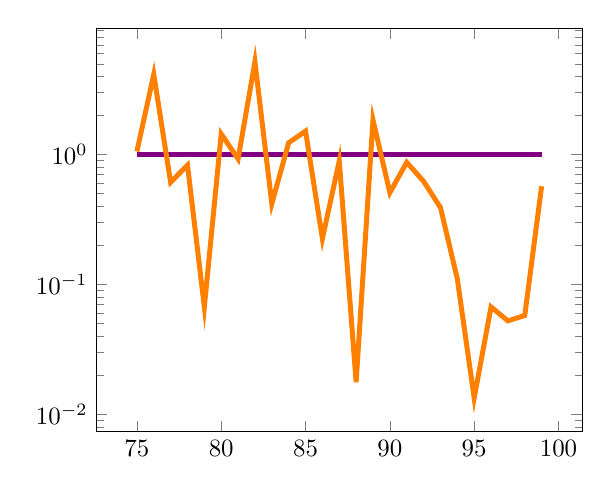
\begin{tikzpicture}[scale=0.9]
\begin{semilogyaxis}
\addplot[color=violet,line width=2pt] coordinates {(75,1.0)(76,1.0)(77,1.0)(78,1.0)(79,1.0)(80,1.0)(81,1.0)(82,1.0)(83,1.0)(84,1.0)(85,1.0)(86,1.0)(87,1.0)(88,1.0)(89,1.0)(90,1.0)(91,1.0)(92,1.0)(93,1.0)(94,1.0)(95,1.0)(96,1.0)(97,1.0)(98,1.0)(99,1.0)};
\addplot[color=orange,line width=2pt] coordinates {(75,1.0559022417429496)(76,4.13758183125973)(77,0.6116797822484966)(78,0.8292564250659684)(79,0.06710056307024373)(80,1.4399041660513077)(81,0.9257927704528695)(82,5.179684560107651)(83,0.4186938508135714)(84,1.2326184699664224)(85,1.515188705688906)(86,0.22549861568331897)(87,0.8924630035417472)(88,0.01768513158965184)(89,1.8444823577468445)(90,0.5091521286012557)(91,0.8704939394965266)(92,0.6220528220757559)(93,0.3911975041811248)(94,0.1105426211436095)(95,0.013335161463880493)(96,0.06705736468394229)(97,0.05237303071920235)(98,0.05765744606925371)(99,0.5699938086567803)};

\end{semilogyaxis}
\end{tikzpicture}
